\documentclass{beamer}
\usetheme{Madrid}
\usecolortheme{dolphin}
\usepackage{amsmath}
\usepackage{graphicx}
\usepackage{hyperref}
\usepackage{tikz}

\title{Introduction to Logic: The Art of Reasoning}
\subtitle{Fundamentals of Logical Thinking}
\author{Brendan Shea, PhD}
\date{\today}

\begin{document}

\begin{frame}
    \titlepage
\end{frame}

\begin{frame}
    \frametitle{Welcome to Logic: The Art of Reasoning}
    \begin{itemize}
        \item Logic is the systematic study of the principles of valid reasoning and argumentation.
        \item Logic provides tools to distinguish good reasoning from poor reasoning.
        \item Logical thinking helps us evaluate claims and make better decisions in everyday life.
        \item This course will develop your ability to recognize, analyze, and construct sound arguments.
    \end{itemize}
    
    \begin{alertblock}{What is Logic?}
        \textbf{Logic} is the study of the methods and principles used to distinguish correct from incorrect reasoning.
    \end{alertblock}
\end{frame}

\begin{frame}
    \frametitle{Why Study Logic? Applications in Daily Life and Academia}
    \begin{itemize}
        \item Logic helps us critically analyze news, advertising, and social media claims.
        \item Logical reasoning is essential for success in many academic disciplines including philosophy, mathematics, computer science, and law.
        \item Clear thinking prevents us from being misled by emotional appeals and fallacious reasoning.
        \item Logic improves our communication by helping us articulate our own thoughts more precisely.
    \end{itemize}
    
    \begin{exampleblock}{Example: Everyday Application}
        When evaluating a product advertisement claiming "9 out of 10 doctors recommend," logic helps us ask important questions: How many doctors were surveyed? What exactly were they asked? Is this a representative sample?
    \end{exampleblock}
\end{frame}

\begin{frame}
    \frametitle{Historical Overview: From Aristotle to Modern Logic}
    \begin{itemize}
        \item Logical study began with Aristotle's systematic analysis of syllogisms in ancient Greece.
        \item Traditional logic remained largely unchanged for nearly 2,000 years until the 19th century.
        \item Modern symbolic logic was developed by mathematicians like George Boole and Gottlob Frege.
        \item Contemporary logic includes modal, temporal, and computational logic systems.
    \end{itemize}
    
    \begin{table}
        \begin{tabular}{|l|l|l|}
            \hline
            \textbf{Period} & \textbf{Key Figures} & \textbf{Contributions} \\
            \hline
            Ancient & Aristotle & Syllogistic logic \\
            \hline
            Medieval & Aquinas, Ockham & Development of temporal logic \\
            \hline
            19th Century & Boole, Frege & Mathematical/symbolic logic \\
            \hline
            20th Century & Russell, Gödel & Modern formal systems \\
            \hline
        \end{tabular}
        \caption{Evolution of Logical Thought}
    \end{table}
\end{frame}

\begin{frame}
    \frametitle{Course Roadmap: What We'll Cover}
    \begin{itemize}
        \item We'll begin by understanding the basic structure of arguments and how to identify them.
        \item We'll explore different types of arguments: deductive, inductive, and abductive reasoning.
        \item We'll learn to distinguish arguments from non-arguments and from explanations.
        \item We'll develop skills to analyze complex arguments and put them in standard form.
    \end{itemize}
    
    \begin{block}{Course Goals}
        \begin{enumerate}
            \item Recognize arguments in everyday language
            \item Evaluate the strength of arguments
            \item Construct your own valid arguments
            \item Apply logical thinking to real-world situations
        \end{enumerate}
    \end{block}
\end{frame}

\begin{frame}
    \frametitle{What Is an Argument? Basic Structure and Purpose}
    \begin{itemize}
        \item An \textbf{argument} is a set of statements where some (the premises) are offered as support for another (the conclusion).
        \item Arguments attempt to provide reasons for accepting a particular claim as true or probable.
        \item Arguments can be expressed in conversation, writing, or even visually through diagrams.
        \item The purpose of an argument is to persuade others to accept a conclusion based on evidence.
    \end{itemize}
    
    \begin{exampleblock}{Simple Argument Example}
        Premise 1: All mammals have lungs.\\
        Premise 2: Whales are mammals.\\
        Conclusion: Therefore, whales have lungs.
    \end{exampleblock}
\end{frame}

\begin{frame}
    \frametitle{Premises: The Foundation of Arguments}
    \begin{itemize}
        \item \textbf{Premises} are statements offered as evidence or reasons to support a conclusion.
        \item Premises can be facts, observations, opinions, or even hypothetical statements.
        \item The quality of premises significantly affects the strength of an entire argument.
        \item Premises may be stated explicitly or left implicit (unstated but assumed).
    \end{itemize}
    
    \begin{alertblock}{Important Note}
        For an argument to be sound, all premises must be true. Even a single false premise can undermine an otherwise logically valid argument.
    \end{alertblock}
\end{frame}

\begin{frame}
    \frametitle{Conclusions: What Arguments Aim to Establish}
    \begin{itemize}
        \item A \textbf{conclusion} is the statement that the argument is trying to prove or support.
        \item The conclusion represents the main point the arguer wants the audience to accept.
        \item Conclusions should follow logically from the premises, though the strength of this connection varies.
        \item A single argument can have only one main conclusion, though it may have sub-conclusions.
    \end{itemize}
    
    \begin{columns}[t]
        \column{0.5\textwidth}
        \textbf{Common Conclusion Indicators:}
        \begin{itemize}
            \item Therefore
            \item Thus
            \item So
            \item Hence
            \item It follows that
        \end{itemize}
        
        \column{0.5\textwidth}
        \textbf{Sometimes Conclusions:}
        \begin{itemize}
            \item Appear at the beginning
            \item Are unstated (implied)
            \item Use no indicator words
            \item Require careful analysis
        \end{itemize}
    \end{columns}
\end{frame}

\begin{frame}
    \frametitle{The Relationship Between Premises and Conclusions}
    \begin{itemize}
        \item The premises of an argument should provide support or justification for the conclusion.
        \item The connection between premises and conclusion is called \textbf{inference}.
        \item The strength of this connection determines whether the argument is strong or weak.
        \item Premises may support a conclusion independently or work together as a unit.
    \end{itemize}
    
    \begin{block}{Two Types of Premise Support}
        \begin{description}
            \item[Independent Support] Each premise provides separate evidence for the conclusion (like multiple witnesses)
            \item[Dependent Support] Premises work together to support the conclusion (like links in a chain)
        \end{description}
    \end{block}
\end{frame}

\begin{frame}
    \frametitle{Indicators: Linguistic Clues for Premises and Conclusions}
    \begin{itemize}
        \item \textbf{Indicator words} are terms that signal the presence of premises or conclusions.
        \item Premise indicators typically appear before statements that provide evidence or reasons.
        \item Conclusion indicators generally appear before statements that express what is being argued for.
        \item Recognizing these indicators helps identify argument structure in complex texts.
    \end{itemize}
    
    \begin{table}
        \begin{tabular}{|l|l|}
            \hline
            \textbf{Premise Indicators} & \textbf{Conclusion Indicators} \\
            \hline
            Because & Therefore \\
            Since & Thus \\
            Given that & Consequently \\
            For the reason that & It follows that \\
            As indicated by & So \\
            \hline
        \end{tabular}
        \caption{Common Indicator Words}
    \end{table}
\end{frame}

\begin{frame}
    \frametitle{Example: Identifying Premises and Conclusions}
    
    \begin{exampleblock}{Spider-Man's Uncle Ben}
    \scriptsize
        "With great power comes great responsibility."
        
        \textbf{Analysis:} This famous quote is actually an enthymeme (argument with unstated premises):
        \begin{itemize}
            \item \textbf{Implied premise 1:} Spider-Man has great power
            \item \textbf{Implied premise 2:} People who have great power have great responsibility
            \item \textbf{Conclusion:} Spider-Man has great responsibility
        \end{itemize}
    \end{exampleblock}
    
    \begin{exampleblock}{Batman's Reasoning}
    \scriptsize
        "The criminal is a coward and superstitious. Therefore, my costume must be terrifying to strike fear in their hearts."
        
        \textbf{Analysis:}
        \begin{itemize}
            \item \textbf{Premise 1:} Criminals are cowardly and superstitious
            \item \textbf{Implied premise 2:} Terrifying symbols strike fear in the cowardly and superstitious
            \item \textbf{Conclusion:} Batman's costume must be terrifying (to be effective)
        \end{itemize}
    \end{exampleblock}
\end{frame}

\begin{frame}
    \frametitle{Distinguishing Arguments from Other Forms of Discourse}
    \begin{itemize}
        \item Not all communication contains arguments—many texts simply inform, describe, or entertain.
        \item An \textbf{argument} specifically attempts to support a claim with reasons or evidence.
        \item Arguments involve both factual claims and logical connections between those claims.
        \item Identifying arguments requires recognizing when someone is trying to convince rather than merely inform.
    \end{itemize}
    
    \begin{exampleblock}{Non-Argument vs. Argument}
        \textbf{Non-Argument:} "The capital of France is Paris. It has many famous landmarks."\\
        \textbf{Argument:} "The capital of France must be Paris because all major guidebooks list it as such, and official government documents identify it as the capital."
    \end{exampleblock}
\end{frame}

\begin{frame}
    \frametitle{Implicit vs. Explicit Arguments}
    \begin{itemize}
        \item \textbf{Explicit arguments} clearly state both premises and conclusion.
        \item \textbf{Implicit arguments} leave some components unstated but implied.
        \item Many real-world arguments contain unstated premises (enthymemes) that are culturally assumed.
        \item Reconstructing implicit arguments requires careful consideration of context and charitable interpretation.
    \end{itemize}
    
    \begin{alertblock}{The Principle of Charity}
        When analyzing arguments, apply the \textbf{principle of charity} by interpreting them in their strongest possible form before evaluation—don't attack "straw man" versions.
    \end{alertblock}
\end{frame}

\begin{frame}
    \frametitle{Argument Indicators in Everyday Language}
    \begin{itemize}
        \item Arguments in everyday conversation often lack formal indicator words.
        \item Questions can sometimes function as implicit conclusions ("Shouldn't we leave now?").
        \item Tone, emphasis, and context provide important clues about argumentative intent.
        \item Professional writing (academic, legal, scientific) tends to use more explicit argument structures.
    \end{itemize}
    
    \begin{block}{Common Contexts for Arguments}
        \begin{itemize}
            \item Persuasive essays and opinion pieces
            \item Political speeches and debates
            \item Academic papers and presentations
            \item Legal proceedings and documents
            \item Everyday disagreements and discussions
        \end{itemize}
    \end{block}
\end{frame}

\begin{frame}
    \frametitle{Finding Hidden Premises and Conclusions}
    \begin{itemize}
        \item Many arguments leave crucial premises unstated because they're assumed to be obvious.
        \item \textbf{Hidden premises} are unstated assumptions necessary for an argument to work.
        \item \textbf{Implied conclusions} must sometimes be inferred from context and content.
        \item Identifying these unstated elements is essential for proper argument evaluation.
    \end{itemize}
    
    \begin{exampleblock}{Argument with Hidden Premise}
        "Maria should take an umbrella because it's going to rain."\\
        \textbf{Hidden premise:} People should take umbrellas when it rains.\\
        \textbf{Stated premise:} It's going to rain.\\
        \textbf{Conclusion:} Maria should take an umbrella.
    \end{exampleblock}
\end{frame}

\begin{frame}
    \frametitle{Deductive Arguments: Aiming for Certainty}
    \begin{itemize}
        \item \textbf{Deductive arguments} aim to provide conclusive support for their conclusions.
        \item In a properly formed deductive argument, if all premises are true, the conclusion must be true.
        \item Deductive arguments move from general principles to specific instances.
        \item Mathematics and formal logic primarily use deductive reasoning.
    \end{itemize}
    
    \begin{alertblock}{Key Concept: Validity}
        A deductive argument is \textbf{valid} if its conclusion must be true when all premises are true. This is about the logical structure, not factual accuracy.
    \end{alertblock}
\end{frame}

\begin{frame}
    \frametitle{Validity and Soundness in Deductive Reasoning}
    \begin{itemize}
        \item A deductive argument can be valid even if its premises are false.
        \item A \textbf{sound} argument is both valid AND has all true premises.
        \item Soundness is the gold standard for deductive arguments—it guarantees a true conclusion.
        \item Evaluating deductive arguments requires checking both structure (validity) and content (truth).
    \end{itemize}
    
    \begin{columns}[t]
        \column{0.5\textwidth}
        \textbf{Valid but Not Sound:}
        
        All fish can fly.\\
        Sharks are fish.\\
        Therefore, sharks can fly.
        
        \column{0.5\textwidth}
        \textbf{Both Valid and Sound:}
        
        All squares have four sides.\\
        This shape is a square.\\
        Therefore, this shape has four sides.
    \end{columns}
\end{frame}

\begin{frame}
    \frametitle{Common Deductive Argument Forms}
    \begin{itemize}
        \item Certain argument patterns are recognized as valid deductive forms.
        \item \textbf{Modus ponens} (If P then Q; P; Therefore Q) is one of the most common valid forms.
        \item \textbf{Modus tollens} (If P then Q; Not Q; Therefore not P) is another reliable form.
        \item Understanding these patterns helps identify valid arguments regardless of content.
    \end{itemize}
    
    \begin{exampleblock}{Modus Ponens Example}
        If it is raining, then the streets are wet. (If P then Q)\\
        It is raining. (P)\\
        Therefore, the streets are wet. (Q)
    \end{exampleblock}
\end{frame}

\begin{frame}
    \frametitle{Inductive Arguments: Reasoning from Evidence to Probability}
    \begin{itemize}
        \item \textbf{Inductive arguments} provide evidence that makes their conclusions probable rather than certain.
        \item Inductive reasoning moves from specific observations to general conclusions.
        \item Science relies heavily on inductive reasoning to formulate theories from data.
        \item The strength of inductive arguments depends on the quality and quantity of evidence.
    \end{itemize}
    
    \begin{block}{Inductive vs. Deductive Reasoning}
        \begin{tabular}{|l|l|}
            \hline
            \textbf{Inductive} & \textbf{Deductive} \\
            \hline
            Specific to general & General to specific \\
            Probabilistic conclusion & Certain conclusion (if valid) \\
            Based on observation & Based on logical necessity \\
            Can add new information & Conclusion contained in premises \\
            \hline
        \end{tabular}
    \end{block}
\end{frame}

\begin{frame}
    \frametitle{Strength and Cogency in Inductive Arguments}
    \begin{itemize}
        \item An inductive argument is \textbf{strong} if its premises make its conclusion probable.
        \item An inductive argument is \textbf{cogent} if it is strong AND all its premises are true.
        \item Strength comes in degrees—inductive arguments can be very strong, moderately strong, or weak.
        \item Adding relevant evidence can strengthen an inductive argument (unlike deductive arguments).
    \end{itemize}
    
    \begin{alertblock}{Important Distinction}
        Inductive arguments are evaluated as \textbf{strong} or \textbf{weak}, not valid or invalid. Using deductive standards for inductive arguments is a common mistake.
    \end{alertblock}
\end{frame}

\begin{frame}
    \frametitle{Common Inductive Reasoning Patterns}
    \begin{itemize}
        \item \textbf{Generalization} draws conclusions about a whole group based on a sample.
        \item \textbf{Analogical reasoning} argues that similar cases should have similar outcomes.
        \item \textbf{Causal reasoning} infers cause-effect relationships from observed correlations.
        \item \textbf{Statistical syllogism} applies group probabilities to individual cases.
    \end{itemize}
    
    \begin{exampleblock}{Inductive Generalization}
        Premise: 95\% of the 1,000 randomly sampled voters support Candidate X.\\
        Conclusion: Therefore, approximately 95\% of all voters likely support Candidate X.
        
        Note: The strength depends on sample size and representativeness.
    \end{exampleblock}
    
\end{frame}

\begin{frame}
    \frametitle{Example: Deductive vs. Inductive Arguments}
    
    \begin{exampleblock}{Superman's Deductive Reasoning}
    \scriptsize
        "All Kryptonians are weakened by Kryptonite. I am a Kryptonian. Therefore, I am weakened by Kryptonite."
        
        \textbf{Analysis:} This is a valid deductive argument (syllogism):
        \begin{itemize}
            \item It has the form: All A are B; C is an A; Therefore, C is B
            \item If the premises are true, the conclusion must be true
            \item The conclusion follows with certainty
        \end{itemize}
    \end{exampleblock}
    
    \begin{exampleblock}{Sherlock Holmes' Inductive Reasoning}
    \scriptsize
        "The last three times Moriarty was in London, a major jewel theft occurred. Moriarty is now in London again. Therefore, another major jewel theft is likely to occur."
        
        \textbf{Analysis:} This is an inductive argument:
        \begin{itemize}
            \item Based on observed pattern of past events
            \item Conclusion is probable but not certain
            \item New evidence could strengthen or weaken it
        \end{itemize}
    \end{exampleblock}
\end{frame}



\begin{frame}
    \frametitle{Abductive Arguments: Inference to the Best Explanation}
    \begin{itemize}
        \item \textbf{Abductive reasoning} seeks the most plausible explanation for observed facts.
        \item It is sometimes called "inference to the best explanation."
        \item Abduction begins with observations and works backward to likely causes.
        \item This form of reasoning is common in medicine, detective work, and scientific discovery.
    \end{itemize}
    
    \begin{exampleblock}{Abductive Reasoning Example}
        Observation: The patio is wet this morning.\\
        Possible explanations: It rained, sprinklers ran, someone washed it.\\
        Best explanation: It rained (most plausible given additional context like wet streets).
    \end{exampleblock}
\end{frame}

\begin{frame}
    \frametitle{Example: Abductive Reasoning}
    
    \begin{exampleblock}{Scooby-Doo Gang's Investigation}
        "The monster only appears when the lighthouse keeper is not around. There are footprints matching the lighthouse keeper's shoes. There's theatrical makeup in the keeper's drawer. The best explanation is that the lighthouse keeper is disguising himself as the monster."
        
        \textbf{Analysis:} Classic abductive reasoning:
        \begin{itemize}
            \item Multiple observations collected (timing, footprints, makeup)
            \item Alternative explanations considered but rejected
            \item Conclusion is the most plausible explanation for all observed facts
            \item Classic "inference to the best explanation"
        \end{itemize}
    \end{exampleblock}
\end{frame}

\begin{frame}
    \frametitle{Comparing the Three Argument Types: When to Use Each}
    \begin{itemize}
        \item \textbf{Deductive arguments} work best when applying established principles to specific cases.
        \item \textbf{Inductive arguments} are appropriate when projecting from observed patterns to new instances.
        \item \textbf{Abductive arguments} are valuable when seeking explanations for phenomena.
        \item Many real-world arguments combine elements of all three types of reasoning.
    \end{itemize}
    
    \begin{table}
        \begin{tabular}{|l|l|l|}
            \hline
            \textbf{Type} & \textbf{Strength} & \textbf{Best Applications} \\
            \hline
            Deductive & Certainty & Mathematics, formal logic, law \\
            \hline
            Inductive & Probability & Science, statistics, forecasting \\
            \hline
            Abductive & Plausibility & Diagnosis, investigation, research \\
            \hline
        \end{tabular}
        \caption{Comparison of Argument Types}
    \end{table}
\end{frame}

\begin{frame}
    \frametitle{Reports: Just the Facts}
    \begin{itemize}
        \item \textbf{Reports} present information without attempting to establish a conclusion.
        \item Reports state what is observed or known without arguing for its truth.
        \item News articles (ideally) report facts without drawing conclusions from them.
        \item Reports may be used within arguments, but are not themselves arguments.
    \end{itemize}
    
    \begin{block}{Characteristics of Reports}
        \begin{itemize}
            \item Focus on observable data
            \item Lack inferential language
            \item Absence of conclusion indicators
            \item Often use neutral, descriptive language
            \item May contain measurements, statistics, or direct quotations
        \end{itemize}
    \end{block}
\end{frame}

\begin{frame}
    \frametitle{Expressions of Opinion: Beliefs Without Support}
    \begin{itemize}
        \item \textbf{Expressions of opinion} state beliefs without providing supporting evidence.
        \item Unlike arguments, they don't attempt to convince through reasons.
        \item Opinions become premises in arguments only when supported by further evidence.
        \item Distinguishing between unsupported opinions and argued positions is crucial for critical thinking.
    \end{itemize}
    
    \begin{columns}[t]
        \column{0.5\textwidth}
        \textbf{Mere Opinion:}\\
        "I believe that jazz is the best form of music."
        
        \column{0.5\textwidth}
        \textbf{Argument:}\\
        "Jazz is the best form of music because it combines technical complexity with emotional expression and allows for individual creativity through improvisation."
    \end{columns}
\end{frame}

\begin{frame}
    \frametitle{Illustrations and Examples: Not Yet Arguments}
    \begin{itemize}
        \item \textbf{Illustrations and examples} provide instances that clarify or elaborate on a concept.
        \item They show rather than prove, though they may be incorporated into arguments.
        \item Concrete examples help understand abstract ideas but don't establish their truth.
        \item Examples become evidence only when used to support generalizations.
    \end{itemize}
    
    \begin{exampleblock}{Illustration vs. Inductive Argument}
        \textbf{Illustration:} "Some birds cannot fly. For instance, penguins and ostriches cannot fly."
        
        \textbf{Inductive Argument:} "Many flightless birds live in environments without predators. Penguins, ostriches, and kiwis all evolved in relatively predator-free environments. Therefore, lack of predators likely contributes to flightlessness in birds."
    \end{exampleblock}
\end{frame}

\begin{frame}
    \frametitle{Expository Passages: Explaining Without Arguing}
    \begin{itemize}
        \item \textbf{Expository passages} aim to explain concepts, processes, or relationships.
        \item They provide information to increase understanding, not to prove a conclusion.
        \item Textbooks, encyclopedias, and instructional materials often use expository writing.
        \item Exposition answers "what," "how," and "why" questions without advocating for claims.
    \end{itemize}
    
    \begin{block}{Clarifying Questions for Distinguishing Exposition from Argument}
        \begin{enumerate}
            \item Is the passage trying to prove something is true?
            \item Or is it explaining how something works or what something means?
            \item Does it assume the truth of what's being discussed?
            \item Is it offering reasons for accepting a conclusion?
        \end{enumerate}
    \end{block}
\end{frame}

\begin{frame}
    \frametitle{Conditional Statements: "If-Then" Without Asserting}
    \begin{itemize}
        \item \textbf{Conditional statements} express relationships between conditions and consequences.
        \item They take the form "If P, then Q" but don't assert that P or Q is actually true.
        \item Conditionals state what would follow if a condition were met.
        \item They become parts of arguments only when the antecedent (the "if" part) is affirmed or the consequent denied.
    \end{itemize}
    
    \begin{exampleblock}{Conditional vs. Argument}
        \textbf{Conditional Statement:} "If it rains, the game will be canceled."
        
        \textbf{Argument Using Conditional:}\\
        "If it rains, the game will be canceled.\\
        It is raining.\\
        Therefore, the game will be canceled."
    \end{exampleblock}
\end{frame}

\begin{frame}
    \frametitle{Arguments vs. Explanations: Key Differences}
    \begin{itemize}
        \item \textbf{Arguments} aim to establish the truth of a claim that is in doubt.
        \item \textbf{Explanations} assume the truth of a claim and clarify why or how it is the case.
        \item Arguments answer "Is it true?" while explanations answer "Why is it true?"
        \item The same set of statements can function as either an argument or explanation depending on context.
    \end{itemize}
    
    \begin{alertblock}{Essential Distinction}
        The key difference is in purpose and what is taken for granted:
        \begin{itemize}
            \item Arguments: The conclusion is in question; premises aim to establish it
            \item Explanations: The phenomenon is accepted as true; the goal is to account for it
        \end{itemize}
    \end{alertblock}
\end{frame}

\begin{frame}
    \frametitle{When Explanations Look Like Arguments}
    \begin{itemize}
        \item Explanations often use the same indicator words as arguments ("because," "since," etc.).
        \item Both explanations and arguments connect statements with inferential relationships.
        \item The difference lies in whether the statement being supported is in doubt or accepted.
        \item Context and the author's purpose are crucial for distinguishing between them.
    \end{itemize}
    
    \begin{columns}[t]
        \column{0.5\textwidth}
        \textbf{Explanation:}\\
        "The bridge collapsed because the supporting cables snapped."\\
        (Assumes bridge collapse is known and explains why)
        
        \column{0.5\textwidth}
        \textbf{Argument:}\\
        "The bridge must have collapsed because several cars were found in the river below."\\
        (Uses evidence to establish that collapse occurred)
    \end{columns}
\end{frame}

\begin{frame}
    \frametitle{Causal Explanations vs. Justifying Reasons}
    \begin{itemize}
        \item \textbf{Causal explanations} describe the mechanisms that brought about an event.
        \item \textbf{Justifying reasons} provide evidence for believing a claim is true.
        \item Causal explanations answer "Why did it happen?" in a factual sense.
        \item Justifying reasons answer "Why should I believe it happened?" in an epistemological sense.
    \end{itemize}
    
    \begin{exampleblock}{Causal vs. Justifying}
        \textbf{Causal Explanation:}\\
        "The water froze because the temperature dropped below 32°F." (physical cause)
        
        \textbf{Justifying Reason:}\\
        "I know the water froze because I observed ice in the container this morning." (evidence for belief)
    \end{exampleblock}
\end{frame}

\begin{frame}
    \frametitle{Example: Argument vs. Explanation}
    
    \begin{exampleblock}{Wonder Woman - Argument}
    \scriptsize
        "The prisoner must be telling the truth because she is bound by the Lasso of Truth, and the Lasso of Truth compels anyone bound by it to speak truthfully."
        
        \textbf{Analysis:} This is an argument:
        \begin{itemize}
            \item It attempts to establish something in doubt (whether the prisoner is telling truth)
            \item It provides evidence/reasons to accept the conclusion
            \item The conclusion is what's being proven
        \end{itemize}
    \end{exampleblock}
    
    \begin{exampleblock}{Wonder Woman - Explanation}
    \scriptsize
        "The prisoner is telling the truth because she is bound by the Lasso of Truth. The Lasso works by magically connecting the bound person to the cosmic essence of truth."
        
        \textbf{Analysis:} This is an explanation:
        \begin{itemize}
            \item It assumes the person is telling the truth (not in doubt)
            \item It explains the mechanism by which the truth-telling occurs
            \item It answers "how" rather than "is it the case"
        \end{itemize}
    \end{exampleblock}
\end{frame}

\begin{frame}
    \frametitle{Identifying the Purpose: Persuasion or Understanding?}
    \begin{itemize}
        \item Context and rhetorical situation help determine if statements aim to persuade or explain.
        \item Arguments attempt to overcome doubt or disagreement about a claim.
        \item Explanations assume agreement about a claim and provide understanding of it.
        \item Ask: "Is the author trying to convince me this is true, or helping me understand why it's true?"
    \end{itemize}
    
    \begin{block}{Contextual Clues}
        Look for these signals to distinguish arguments from explanations:
        \begin{itemize}
            \item Is the claim controversial or accepted?
            \item Is the audience likely to doubt the claim?
            \item Does the communication aim to resolve disagreement?
            \item Does the author treat the main claim as established or in need of support?
        \end{itemize}
    \end{block}
\end{frame}

\begin{frame}
    \frametitle{What Is Standard Form and Why Use It?}
    \begin{itemize}
        \item \textbf{Standard form} presents arguments with premises clearly listed and the conclusion identified.
        \item It eliminates rhetorical flourishes and focuses on the logical structure.
        \item Standard form helps identify missing premises and evaluate logical connections.
        \item Converting arguments to standard form is a crucial skill for critical analysis.
    \end{itemize}
    
    \begin{exampleblock}{Natural Language vs. Standard Form}
        \textbf{Natural language:}\\
        "Since smoking damages the lungs and heart and increases cancer risk, anyone concerned about their health should avoid cigarettes."
        
        \textbf{Standard form:}\\
        P1: Smoking damages the lungs and heart.\\
        P2: Smoking increases cancer risk.\\
        P3: People should avoid behaviors that damage health.\\
        C: Anyone concerned about their health should avoid cigarettes.
    \end{exampleblock}
\end{frame}

\begin{frame}
    \frametitle{Step 1: Identifying All Premises and the Conclusion}
    \begin{itemize}
        \item The first step is to carefully read the entire argument to understand its overall point.
        \item Identify the conclusion—the main claim the argument is trying to establish.
        \item Look for indicator words that signal premises and conclusions.
        \item Watch for premises that are stated in questions or commands rather than declarative sentences.
    \end{itemize}
    
    \begin{alertblock}{Common Challenge}
        Many everyday arguments have multiple conclusions, with some serving as intermediate steps (sub-conclusions). Identify the main conclusion first, then work backward to find supporting premises.
    \end{alertblock}
\end{frame}

\begin{frame}
    \frametitle{Step 2: Eliminating Irrelevant Material}
    \begin{itemize}
        \item Arguments often contain material that doesn't directly support the conclusion.
        \item \textbf{Rhetorical flourishes} add persuasive force but not logical support.
        \item \textbf{Repetition} may emphasize points but doesn't add new support.
        \item \textbf{Tangential information} might be interesting but irrelevant to the logical structure.
    \end{itemize}
    
    \begin{exampleblock}{Identifying Relevant Content}
        Original: "As any sensible person can clearly see, and as experts have repeatedly confirmed beyond any shadow of doubt, excessive sugar consumption leads to health problems. Sugar is in everything these days! Therefore, reducing sugar intake is essential for maintaining good health."
        
        Relevant content only:
        P1: Excessive sugar consumption leads to health problems.
        C: Reducing sugar intake is essential for maintaining good health.
    \end{exampleblock}
\end{frame}

\begin{frame}
    \frametitle{Step 3: Arranging Premises Logically}
    \begin{itemize}
        \item After identifying premises and conclusions, arrange them in logical order.
        \item Identify \textbf{suppressed premises} that are implied but not stated.
        \item Group related premises that work together to support a sub-conclusion.
        \item Number premises and clearly mark the conclusion.
    \end{itemize}
    
    \begin{block}{Approaches to Arrangement}
        Two common ways to arrange premises:
        \begin{enumerate}
            \item \textbf{Linear arrangement:} Each premise builds on previous ones toward the conclusion
            \item \textbf{Branching arrangement:} Multiple independent lines of support for the conclusion
        \end{enumerate}
    \end{block}
\end{frame}

\begin{frame}
    \frametitle{Practice: Converting Real-World Arguments to Standard Form}
    \begin{itemize}
        \item Converting real arguments requires practice and careful reading.
        \item Different readers may produce slightly different standard forms of the same argument.
        \item The goal is to capture the logical essence of the argument faithfully.
        \item Standard form should clarify, not distort, the original argument's intent.
    \end{itemize}
    
    \begin{exampleblock}{Practice Example}
    \scriptsize
        Original text: "Free college education should be available to all qualified students. After all, an educated population benefits society through increased productivity and innovation. Furthermore, making higher education dependent on wealth perpetuates inequality."
        
        Standard form:\\
        P1: An educated population benefits society through increased productivity and innovation.\\
        P2: Making higher education dependent on wealth perpetuates inequality.\\
        P3: (Implied) Society should maximize benefits and reduce inequality.\\
        C: Free college education should be available to all qualified students.
    \end{exampleblock}
\end{frame}

\begin{frame}
    \frametitle{Example: Hidden Premises}
    
    \begin{exampleblock}{Popeye's Reasoning}
    \scriptsize
        "I need to be strong. Therefore, I must eat spinach."
        
        \textbf{Analysis:} This enthymeme has multiple hidden premises:
        \begin{itemize}
            \item \textbf{Stated premise:} I need to be strong
            \item \textbf{Hidden premise 1:} Spinach makes me strong
            \item \textbf{Hidden premise 2:} If I need to be strong and spinach makes me strong, then I should eat spinach
            \item \textbf{Conclusion:} I must eat spinach
        \end{itemize}
    \end{exampleblock}
    
    \begin{exampleblock}{Captain America's Appeal}
    \scriptsize
        "The Sokovia Accords restrict our freedom to act. Therefore, we should oppose them."
        
        \textbf{Analysis:} Hidden value premise:
        \begin{itemize}
            \item \textbf{Stated premise:} The Sokovia Accords restrict freedom to act
            \item \textbf{Hidden premise:} Restrictions on freedom to act (for superheroes) are harmful/wrong
            \item \textbf{Hidden premise:} We should oppose harmful/wrong policies
            \item \textbf{Conclusion:} We should oppose the Sokovia Accords
        \end{itemize}
    \end{exampleblock}
\end{frame}


\begin{frame}
    \frametitle{Breaking Down Extended Arguments}
    \begin{itemize}
        \item \textbf{Extended arguments} contain multiple inferences leading to a main conclusion.
        \item These arguments often have a hierarchical structure with sub-arguments.
        \item Break down complex arguments by identifying intermediate conclusions.
        \item Analyze each sub-argument individually before examining how they work together.
    \end{itemize}
    
    \begin{exampleblock}{Extended Argument Structure}
        P1: Studies show that exercise increases endorphin production.\\
        P2: Increased endorphin production improves mood.\\
        SC1: Therefore, exercise improves mood.\\
        
        P3: Improved mood reduces stress.\\
        P4: Reduced stress strengthens immune function.\\
        MC: Therefore, exercise strengthens immune function.
        
        (where SC1 = sub-conclusion, MC = main conclusion)
    \end{exampleblock}
\end{frame}

\begin{frame}
    \frametitle{Argument Maps: Visualizing Reasoning Structures}
    \begin{itemize}
        \item \textbf{Argument maps} are visual diagrams showing logical relationships between statements.
        \item They use boxes for claims and lines/arrows to indicate support relationships.
        \item Mapping reveals the overall structure of an argument at a glance.
        \item Maps help identify weak points and understand how parts of an argument relate.
    \end{itemize}
    
    \begin{figure}
        \centering
        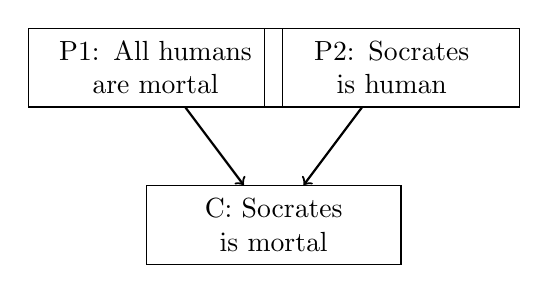
\begin{tikzpicture}[
            box/.style={rectangle, draw, text width=3cm, align=center, minimum height=1cm},
            arrow/.style={->, thick}
        ]
            \node[box] (p1) at (0,0) {P1: All humans are mortal};
            \node[box] (p2) at (3,0) {P2: Socrates is human};
            \node[box] (c1) at (1.5,-2) {C: Socrates is mortal};
            
            \draw[arrow] (p1) -- (c1);
            \draw[arrow] (p2) -- (c1);
        \end{tikzpicture}
        \caption{Simple Argument Map}
    \end{figure}
\end{frame}

\begin{frame}
    \frametitle{Sub-arguments and Chains of Reasoning}
    \begin{itemize}
        \item \textbf{Sub-arguments} are smaller arguments that support premises in the main argument.
        \item A \textbf{chain of reasoning} occurs when conclusions become premises for further arguments.
        \item The strength of each link affects the overall strength of the argument chain.
        \item Complex arguments often blend multiple types of reasoning (deductive, inductive, abductive).
    \end{itemize}
    
    \begin{alertblock}{Critical Insight}
        In a chain of reasoning, the conclusion is only as strong as the weakest link. If any step in the chain is flawed, subsequent conclusions become questionable, even if their immediate inferences are valid.
    \end{alertblock}
\end{frame}

\begin{frame}
    \frametitle{Logic in Action: Applying What We've Learned}
    \begin{itemize}
        \item Logic isn't just an academic exercise—it's a practical tool for everyday reasoning.
        \item Recognizing argument structures helps evaluate news, advertisements, and political discourse.
        \item Constructing good arguments improves your ability to communicate and persuade effectively.
        \item Critical thinking skills developed through logical analysis transfer to all areas of life.
    \end{itemize}
    
    \begin{block}{Key Takeaways}
        \begin{itemize}
            \item Arguments provide reasons to accept conclusions
            \item Different types of arguments serve different purposes
            \item Standard form clarifies logical structure
            \item Complex arguments can be broken down into components
            \item Logic improves both our thinking and communication
        \end{itemize}
    \end{block}
\end{frame}



\end{document}